\documentclass[11pt,letterpaper]{article}
\usepackage[margin=1in]{geometry}
\usepackage{amsmath,amsthm}
\usepackage{newtxtext,newtxmath}
\usepackage{booktabs,graphicx,microtype,xcolor}
\usepackage[numbers,sort&compress]{natbib}
\usepackage[colorlinks=true,allcolors=blue!45!black]{hyperref}
\usepackage{fancyhdr}
\pagestyle{fancy}\fancyhf{}\fancyhead[L]{\small Sparse titration and decision reliability}\fancyhead[R]{\small Gupta}\fancyfoot[C]{\thepage}
\setlength{\headheight}{14pt}
\setlength{\emergencystretch}{2em}
\newtheorem{proposition}{Proposition}
\newtheorem{theorem}{Theorem}
\newcommand{\KD}{K_{\mathrm D}}
\newcommand{\ind}{\mathbf 1}
\newcommand{\method}{\textsc{TitraSelect}}
\newcommand{\PrimaryRuns}{840}
\newcommand{\ContrastCoverageRange}{10.4\% to 90.0\%}
\newcommand{\RawFlipRange}{16.0--39.3\%}
\newcommand{\ResultsCoverage}{The selected contrast certifies 81.8\% coverage on CR6261--H1, 77.9\% on CH65--MA90, and 77.3\% on CH65--G189E. It reaches only 10.4\% on CR9114--H3 and 17.4\% on CR6261--H9. The published full-curve fits reach 92.5\% and 28.9\% on the first and fourth tasks, respectively. The sparse rule therefore offers a useful tradeoff in some settings and a substantial loss in others. No primary run has aggregate accepted error above 10\% (0/840 violations); empty acceptance sets are excluded from error averages. This observed statement does not replace the probabilistic guarantee or establish simultaneous coverage for all runs. All eight methods defer on the influenza-B cohorts, which contain only 115--149 evaluable variants. Their calibration subsets contain at most 44 variants before class-specific acceptance, leaving insufficient evidence under the declared correction.}
\newcommand{\ResultsRecall}{On CH65--SI06, the fixed three-point rule covers 98.7\% of the evaluable test cohort with 2.1\% accepted error, but retains only 29.8\% of reference hits for further testing. The raw full-panel learner retains 95.7\% at 92.6\% coverage. No method positively identifies any test hit on CH65--SI06 or CR9114--H1 after class-specific calibration; its retained hits, where present, are deferred rather than declared discoveries. The hit-protection variant makes this distinction operational. With the same 300-variant calibration cap, every method defers completely on CH65--SI06. It has no observed class-error or hit-loss violation in its 504 method--split runs, but often achieves this by sharply reducing negative acceptance. Appendix tables report positively identified hits and hits retained separately.}
\newcommand{\ResultsStress}{The constructed test-only transformations change 16.0--39.3\% of forced decisions across raw-input method/task means. Both the learned three-point ratio and the full-panel invariant learner have zero decision changes in all reported runs. The standardized contrast also preserves its decisions and acceptance set when its linear-space spreads transform consistently. Raw learners can violate their original accepted-error target after the shift; this is an expected failure of transporting a calibration certificate outside its conditions, not a counterexample to the theorem.}
\newcommand{\ResultsSensitivity}{Changing the calibration cap from 100 to 1,000 variants changes which gates can be certified, without changing the physical number of source conditions. Changing the cutoff by half a log unit changes both reference prevalence and the comparison being asked. The supplementary tables include every declared sensitivity setting, including 5\% and 20\% error targets; no setting is omitted because its coverage is zero. The retained-hit analysis additionally shows that a 10\% accepted-error target and a 10\% discarded-hit target are materially different objectives.}
\newcommand{\VerificationText}{Independent data alignment reconstructs stored fit $r^2$ for 18,475 high-quality source curves across all 21 tables; the maximum absolute discrepancy is 5.45e-10. The verification suite checks 55,000 noiseless contrast signs under varied affinities, amplitudes, backgrounds, and affine transforms. It exhaustively checks exact bound coverage in 6,273 finite-population settings, and verifies that changing held-out test labels leaves decisions and calibration gates unchanged. These checks establish implementation properties under their stated inputs, not wet-lab validity of the response model.}

\title{When Can a Sparse Titration Replace a Full Curve?\\[4pt]\large Affine-Invariant Screening with Finite-Library Error Control}
\author{Shivam Gupta\\\small Independent Researcher\\\small\texttt{shivam1720406@gmail.com}}
\date{17 October 2026}
\begin{document}
\maketitle
\begin{abstract}
Protein-discovery systems must decide not only which molecules to test, but which measurements justify a biological decision. We study replacing a full binding titration by a blank and two antigen concentrations for the specific decision $\KD\leq\tau$. A three-point contrast eliminates unknown additive background and multiplicative amplitude under a one-site binding model. An exact finite-population audit then certifies the error among accepted positive and negative decisions separately, with explicit abstention and no independence assumption between related genotypes. We evaluate mechanistic, isotonic, and tree-based readouts using measured titration data from two published studies, three antibody families, eight antibody--antigen tasks, and 21 source/reference configurations. The evaluation contains \PrimaryRuns\ primary method--split runs. Three-point screening is useful in some configurations but does not uniformly replace full curves: mean certified coverage of the selected mechanistic rule ranges from \ContrastCoverageRange\ across tasks with nonzero coverage, and all methods defer on the small evaluable influenza-B cohorts. Learned raw-signal predictors can achieve greater unshifted coverage but change \RawFlipRange\ of decisions under a constructed test-only affine perturbation; ratio-based predictors preserve decisions. A second certificate bounds the fraction of reference hits discarded as negatives, exposing the cost of protecting rare binders. The contribution is a reproducible, decision-specific assay-compression benchmark and an auditable measurement workflow. It does not establish a new binding assay, new antibody mechanism, or prospective laboratory cost savings.
\end{abstract}
\noindent\textbf{Keywords:} experimental design; antibody affinity; titration; selective prediction; finite-population inference; scientific discovery.

\section{Introduction}
An automated discovery system can propose a productive sequence and still choose an inadequate experiment. A large binding signal can reflect affinity, expression, background, or a combination of these quantities. Conversely, measuring a complete curve for every candidate may spend resources on parameters that a particular decision does not require. The appropriate question is therefore operational: \emph{which measurements suffice for a specified biological decision, and when should the system request more evidence?}

We study the decision that a variant's dissociation constant is below a declared threshold. This is a screening decision, distinct from recovering the full kinetic or thermodynamic behavior of an interaction. Tite-Seq already separates affinity from expression by measuring multiple concentrations \citep{adams2016}. Sparse screening is also established commercially: a binding service offers a two-concentration screen separately from fuller affinity characterization \citep{adaptyv}. Neither sparse measurement nor expression confounding is the novelty claimed here.

The unresolved practical issue addressed in this study is the joint behavior of compression, nuisance invariance, and validation. A sparse predictor may exploit a correlation between expression and affinity in a particular library. Its accuracy then need not survive an expression change. A mechanistic invariant may avoid this shortcut but perform poorly when observations are noisy or the model is inadequate. Finally, a prediction can be accurate on average while a small calibration sample cannot certify its accepted decisions. These are different failure modes and require different tests.

We introduce \method, an implementation of a deliberately limited measurement workflow. It selects two positive concentrations using development variants, computes an affinity contrast or an invariant ratio, and validates acceptance gates by exact sampling-without-replacement inference. It returns positive, negative, or defer. We compare it with equally budgeted learned readouts, full-panel learned predictors, and the original full-curve fits. Biological replicates provide reference outcomes; affine perturbations are analyzed separately as constructed robustness tests. The full protocol and numerical results are available with the code \citep{artifact}.

Our contributions are: (i) a concrete affinity-decision formulation with an algebraically auditable nuisance-invariant readout; (ii) finite-library error control for selected gates, including the validation cost that makes some settings infeasible; and (iii) a cross-replicate benchmark on eight measured tasks that reports both successful compression and complete deferral. The algebra and statistical ingredients are applications of established binding models and risk-control principles. The empirical comparison and their integration into this measurement workflow are the research contributions.

\section{Related work and scope of novelty}
\paragraph{Quantitative binding landscapes.}
Tite-Seq measures sequence--affinity landscapes using titration rather than treating enrichment as affinity \citep{adams2016}. Subsequent work analyzed epistasis in the 4-4-20 antibody landscape \citep{adams2019}. The two studies reused here measured combinatorial landscapes for CR6261 and CR9114, and for CH65 \citep{phillips2021,phillips2023}. Their scientific targets concern the evolution and epistasis of binding breadth. Our target is the reliability of a compressed measurement decision. We introduce no new antibody sequence or experimentally verified binding mechanism.

\paragraph{Optimal design and active protein learning.}
Optimal design for saturating response models predates modern protein language models \citep{dette1999}. EVOLVEpro couples protein representations with iterative experimental feedback \citep{evolvepro}; ProSpero studies sequence exploration using an updated surrogate \citep{prospero}. These approaches primarily prioritize sequences. Our action space is a shared measurement panel and a decision gate for an existing finite library. We do not compare discovery rates against these systems because the present experiment neither proposes unmeasured variants nor executes a prospective design cycle. Protein uncertainty benchmarks also show that uncertainty performance depends on task and distribution shift \citep{greenman2025}; we accordingly evaluate accepted errors rather than interpreting a heuristic spread as a calibrated confidence interval.

\paragraph{Prediction with abstention and risk control.}
Risk-controlling prediction sets and Learn then Test validate decision rules using held-out outcomes \citep{bates2021,angelopoulos2021}. Sampling-without-replacement inference can provide guarantees for a fixed population without modeling dependence among its members \citep{waudby2020}. Protein-specific risk control is also established: CPEC controls function-annotation false discoveries, and conformal protein retrieval addresses discovery and missed-match losses \citep{ding2024,boger2025}. Feedback covariate shift in biomolecular design has its own conformal treatment \citep{fannjiang2022}. The present work concerns measured assay panels and fixed-library reference decisions, rather than inventing risk control for protein discovery. Our fixed-time hypergeometric inversion is a classical construction, not a new general risk-control theorem. Its use here separates errors among accepted affinity hits and accepted non-hits, and makes the guarantee refer to the unvalidated remainder of the current library.

A targeted search through 17 October 2026 covered Tite-Seq compression, sparse affinity measurement, binding optimal design, protein active learning, and finite-population risk control. It did not identify the same cross-replicate comparison with these decision gates. This is a scoped novelty assessment, not an exhaustive priority or patentability claim. The closest precedents and the distinctions above are essential to interpreting the contribution.

\section{Decision model and invariant readouts}
\subsection{A biological decision rather than a full parameter estimate}
Let $c$ be antigen concentration and let $F(c)$ be the response in linear fluorescence units. Consider the standard one-site model
\begin{equation}
 F(c)=B+A\frac{c}{K+c},\qquad A>0,\quad B\geq0,\quad K>0.
 \label{eq:binding}
\end{equation}
Here $K$ is the dissociation constant, $A$ is the dynamic amplitude, and $B$ is the background. The desired label is $Y=\ind\{K\leq\tau\}$. The threshold $\tau$ is a screening specification; it is not a universal criterion of therapeutic usefulness.

A single positive concentration cannot identify this label when $A$ is unrestricted. Even if $B$ is known, any $K>0$ can produce a fixed response $f>B$ by choosing $A=(f-B)(K+c)/c$. A second positive concentration with unknown $B$ also leaves a continuum of compatible parameters in general. Additional assumptions, informative priors, or supervised correlations can still make such screens predictive. The non-identifiability statement concerns unrestricted recovery from the response model, not empirical prediction within a fixed library.

\subsection{A three-point threshold contrast}
Take a blank and two positive concentrations $0<c_\ell<c_h$. Define
\begin{equation}
 q_\tau=\frac{c_\ell(\tau+c_h)}{c_h(\tau+c_\ell)},\qquad
 D_\tau=F(c_\ell)-q_\tau F(c_h)-(1-q_\tau)F(0).
 \label{eq:contrast}
\end{equation}
Since $0<q_\tau<1$, this is a background-canceling linear contrast.

\begin{proposition}[Decision equivalence and affine invariance]
Under Eq.~\eqref{eq:binding},
\begin{equation}
 D_\tau=\frac{A c_\ell(c_h-c_\ell)(\tau-K)}{(K+c_\ell)(K+c_h)(\tau+c_\ell)}.
 \label{eq:factor}
\end{equation}
Consequently, $D_\tau\geq0$ if and only if $K\leq\tau$. For any variant-specific transformation $F'(c)=aF(c)+b$ with $a>0$ constant across concentrations, $D'_\tau=aD_\tau$.
\end{proposition}
\begin{proof}
The coefficients of $B$ in Eq.~\eqref{eq:contrast} sum to zero. Substituting $Ac/(K+c)$ and collecting terms yields Eq.~\eqref{eq:factor}; all factors in its denominator are positive. The coefficients also sum to zero for an added $b$, while multiplication by $a$ factors out.
\end{proof}

For noisy responses $\widetilde F$, the sign need not equal the affinity label. If deterministic bounds $|\widetilde F_j-F_j|\leq e_j$ were available, then
\begin{equation}
 |D_\tau(\widetilde F)-D_\tau(F)|\leq e_\ell+q_\tau e_h+(1-q_\tau)e_0.
 \label{eq:noise}
\end{equation}
We do not assume that the reported experimental spreads are such bounds. Instead, their first-order linear-space propagation supplies a ranking scale $s_j=(\ln10)10^{y_j}\sigma_j$ for log-response $y_j$. The mechanistic score is $D_\tau/(s_\ell+q_\tau s_h+(1-q_\tau)s_0)$. Its reliability is assessed against independent reference outcomes.

A complementary readout is
\begin{equation}
 R=\frac{\widetilde F(c_\ell)-\widetilde F(0)}{\widetilde F(c_h)-\widetilde F(0)}.
 \label{eq:ratio}
\end{equation}
The ratio is invariant to positive affine transformations whenever its denominator is positive. Under the noiseless model, $R\geq q_\tau$ is the same decision. An isotonic map fitted on development variants can learn a monotone relation between $R$ and cross-replicate labels, allowing a library-specific decision boundary. This learned boundary sacrifices the exact mechanistic interpretation of the zero contrast but retains the ratio's algebraic invariance. Ratios are clipped to $[0,1]$; nonpositive dynamic ranges receive a fixed value of $1/2$. These rules are declared before calibration.

\begin{figure}[t]
\centering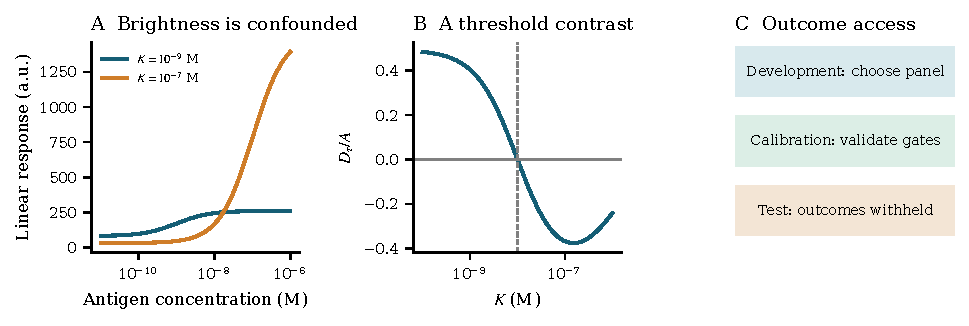
\includegraphics[width=\linewidth]{figures/geometry.pdf}
\caption{Decision geometry and the separation of evidence. Left: illustrative one-site curves, with different amplitudes and backgrounds. These curves are mathematical examples, not experimental observations. Center: the sign of the threshold contrast depends on affinity under the model. Right: development outcomes choose a panel; a separate random calibration subset validates gates; the remaining reference outcomes are withheld from both steps.}
\label{fig:geometry}
\end{figure}

\section{Exact validation on the remaining library}
\subsection{The object that is certified}
After development, let the remaining evaluable library be a fixed finite population. Each variant has a fixed reference label, predicted class, and score. No independence among genotypes, mutations, or measurements is required. Randomness enters through a simple random calibration sample, drawn without replacement from this population. All remaining source-panel features may be observed; their reference labels may not be used to select the score or gate.

For a fixed gate $g$ and predicted class $z\in\{0,1\}$, let $M_g$ denote the number of accepted variants in calibration plus test, $n_g$ the accepted calibration count, and $k_g$ its observed error count. If $E_g$ is the fixed total number of errors in that accepted population, then, conditional on $n_g$,
\begin{equation}
 k_g\sim\operatorname{Hypergeom}(M_g,E_g,n_g).
\end{equation}
For $\eta>0$, define
\begin{equation}
 U_E=\max\left\{E\in\{k_g,\ldots,M_g-n_g+k_g\}:\Pr_E(X\leq k_g)>\eta\right\}.
\end{equation}
The upper bound on the error fraction among accepted \emph{test} variants is
\begin{equation}
 U_g=\frac{U_E-k_g}{M_g-n_g}.
 \label{eq:remaining}
\end{equation}
An unsampled, nonempty accepted population receives bound one. Empty test populations are never selected as useful gates.

\begin{theorem}[Selected finite-library gate]
Suppose each of the two predicted classes has at most $L$ fixed candidate gates, determined without calibration or test reference labels. Use Eq.~\eqref{eq:remaining} with $\eta=\delta/(2L)$. Select any gate per class with $U_g\leq\alpha$, or defer on that class if none qualifies. With probability at least $1-\delta$ over calibration sampling, the error fraction among accepted test variants in each nonempty predicted class is at most $\alpha$. The combined accepted error fraction is then at most $\alpha$.
\end{theorem}
\begin{proof}
For a fixed $E$, its lower-tail cumulative probability evaluated at $X$ is a super-uniform discrete $p$-value. Thus the event $U_E<E$ has probability at most $\eta$. Subtracting the observed $k_g$ and dividing by the fixed realized test count gives the bound on the remaining errors. This argument holds conditional on each accepted calibration count. A union bound covers both classes and every candidate gate, so subsequent gate selection cannot invalidate the simultaneous event. A weighted average of two class-specific error fractions bounded by $\alpha$ is also bounded by $\alpha$.
\end{proof}

This guarantee concerns the recorded reference labels in the defined finite library. It does not identify latent biological truth, guarantee recall, or transfer automatically to a new library or experimental day. Positive-class error is false discovery among accepted hits; negative-class error is false omission among accepted non-hits. These are not the false-positive and false-negative rates conditional on the true class.

\subsection{Validation has a nonzero minimum cost}
Even an error-free calibration sample may be too small. Write $d=M-n>0$ and suppose $k=0$. The smallest total error count violating the test-risk target is $E_0=\lfloor\alpha d\rfloor+1$. Zero observed errors can rule out this count only when
\begin{equation}
 \Pr_{E_0}(X=0)=\frac{\binom{M-E_0}{n}}{\binom{M}{n}}\leq\frac{\delta}{2L}.
 \label{eq:debt}
\end{equation}
For a large population and a small sampling fraction, this probability approaches $(1-\alpha)^n$. At $\alpha=0.1$, $\delta=0.05$, and $L=20$, about 64 accepted, error-free calibration observations are needed in that approximation. The requirement is per accepted class, not per total calibration sample. Rare outcomes, class imbalance, and multiple candidate gates therefore reduce the useful coverage obtainable from a fixed reference budget.

\subsection{Protecting hits that would otherwise be discarded}
A low false-omission fraction does not protect rare hits: predicting every variant negative has small negative-class error whenever hits are rare. For discovery triage, a more relevant requirement is to retain true hits among the positive or deferred variants.

Fix a candidate negative gate. Let $V$ be the number of true reference hits among its accepted test negatives, and let $W$ be the number among all other test variants. The fraction of reference hits discarded is $V/(V+W)$, defined as zero when no reference hit exists. Hypergeometric inversion gives an upper count bound $U_-$ on $V$. On the complementary source-defined stratum, invert the count of negative labels to obtain a lower count bound $L_+$ on $W$. On the joint confidence event,
\begin{equation}
 \frac{V}{V+W}\leq H_g:=\frac{U_-}{U_-+L_+},
 \label{eq:protect}
\end{equation}
with $H_g=0$ when $U_-=0$ and $H_g=1$ when $U_->0,L_+=0$. This follows because $v/(v+w)$ increases in $v$ and decreases in $w$. No independence between the two strata is needed.

The hit-protection variant requires both $U_g\leq\alpha$ and $H_g\leq\alpha$ for a negative gate. Positive gates retain their original condition. We use the conservative common tail level $\delta/(4L)$ for all count bounds, covering the original gates and the complementary-stratum bounds simultaneously. A union-bound argument then gives both accepted-class error control and at most an $\alpha$ fraction of discarded reference hits, with probability at least $1-\delta$. If no negative gate qualifies, all such decisions defer and no reference hit is discarded by that gate. This certificate protects retention for further experiments; it does not guarantee that retained hits have already been positively identified.

\section{Measured-data evaluation}
\subsection{Studies, assay grids, and reference outcomes}
We use public processed Tite-Seq observations from Phillips et al.~\citep{phillips2021} and Phillips et al.~\citep{phillips2023}, pinned to repository commits listed in Appendix~\ref{app:repro}. The first study supplies CR6261--H1/H9 and CR9114--H1/H3/influenza-B tasks, each with three biological replicates. The second supplies CH65--MA90/SI06/G189E tasks, each with two replicates. Theoretical library sizes are 2,048 for CR6261 and 65,536 for each other family. The first study contains 12 binding conditions including a blank; CH65 contains 10.

Each replicate becomes the source once, producing 21 source/reference configurations. For the three-replicate study, the reference label thresholds the mean clipped $-\log_{10}\KD$ from the other two days. Both reference fits must have $r^2\geq0.8$ and reported log-affinity standard deviation at most one. For CH65, the sole other replicate supplies the reference under the same fit-quality requirements. Source curves must have finite responses and positive finite reported spreads at every condition. These complete-case restrictions define the \emph{evaluable cohort}; they are shared by all methods. The reference restrictions cannot be known prospectively without reference measurements. Cases outside this cohort are unresolved, rather than valid negative examples.

We use the authors' target-specific inference grids, not rounded nominal doses. For the first study, the highest log-concentrations are $-7.05$ for H1, $-7.02$ for H9, $-5.95$ for H3, and $-5.87$ for influenza B, followed by half-log steps. CH65 grids come directly from sample metadata. For CH65--MA90 replicate a, we use the authors' corrected table, which removes spurious counts associated with a missing library fragment. The CH65 export rotates response columns by one position; we explicitly undo that rotation. We reproduce stored fit $r^2$ values from the supplied parameters to verify concentration and column alignment. The physical blank is modeled as zero; the original fit code's numerical substitutes for zero are retained only in that alignment check.

The operational log-affinity cutoffs are 9.0 for CR6261, 9.5 for CR9114--H1, 7.0 for CR9114--H3/influenza-B, and 9.0 for CH65. These exploratory cutoffs were chosen after inspecting cohort summaries and are not preregistered. Sensitivity analyses shift them by $\pm0.5$ log units. Results must therefore be interpreted as measured retrospective screening tasks, not prospective validation of a universal affinity threshold.

\begin{table}[t]
\centering\footnotesize
\caption{Evaluable cohorts across source/reference configurations. Ranges reflect source day. Evaluable fractions refer to the source library; positive fractions refer to the restricted cohort. The cut is on $-\log_{10}K_{\mathrm D}$.}
\setlength{\tabcolsep}{4pt}
\begin{tabular}{lrrrr}
\toprule
Task & $N$ & Evaluable (\%) & Reference hits (\%) & Cut \\
\midrule
CR6261-H1 & 1,557--1,619 & 76.03--79.05 & 64.2--67.0 & 9.0 \\
CR6261-H9 & 1,251--1,337 & 61.08--65.28 & 69.4--92.9 & 9.0 \\
CR9114-H1 & 61,514--61,774 & 93.86--94.26 & 14.7--27.8 & 9.5 \\
CR9114-H3 & 5,596--6,625 & 8.54--10.11 & 49.9--58.3 & 7.0 \\
CR9114-FluB & 115--149 & 0.18--0.23 & 73.7--78.3 & 7.0 \\
CH65-MA90 & 61,424--61,427 & 93.73--99.98 & 76.4--79.2 & 9.0 \\
CH65-SI06 & 34,891--34,906 & 53.24--53.26 & 2.4--3.7 & 9.0 \\
CH65-G189E & 61,681--62,025 & 94.12--94.64 & 43.8--44.9 & 9.0 \\
\bottomrule
\end{tabular}
\end{table}


\subsection{Splits, methods, and calibration}
For each configuration and seed, a random permutation selects $\min(200,\lfloor0.2N\rfloor)$ development variants, then $\min(300,\lfloor0.3N\rfloor)$ calibration variants, leaving the rest for testing. The five primary seeds are 1720--1724. Development and calibration membership are disjoint. A tested variant's reference label never contributes to model fitting, panel selection, or gate selection. The random split estimates performance on the remainder of the same finite library; it is not a claim of sequence-distance generalization.

The selected contrast searches all two-positive-concentration pairs (55 for 12-condition assays, 36 for CH65) and minimizes development balanced error, with a deterministic index tie-break. Every pair also uses the blank. The fixed contrast uses the highest concentration and the grid point nearest $\tau$. The learned ratio uses the selected pair and fits isotonic regression to its blank-subtracted ratio.

Learned raw-panel baselines use extremely randomized trees on either the selected three log-responses or the full panel. A full-panel invariant baseline uses blank-subtracted ratios normalized by the highest-concentration response. A one-condition baseline uses the concentration nearest $\tau$. All tree classifiers use 100 trees, maximum depth eight, minimum leaf size five, balanced class weights, and the split seed. The final comparator is the authors' source full-curve affinity fit, scored by its distance from the threshold divided by the reported fit uncertainty, floored at 0.05. Missing source fits receive zero confidence; they are not removed from the cohort.

For every method, predicted positive and negative classes have separate acceptance gates. The grid contains 20 development-margin quantiles from zero to 0.95. Gates are tested at $\alpha=0.10$, $\delta=0.05$, with a correction for 40 candidates. Among qualifying gates, the rule maximizes the number of accepted test variants using only their source features. The probability guarantee applies separately to each method, source configuration, and split, not simultaneously to the complete experiment table. We report task-macro means over source configurations and split seeds, with no claim that overlapping resamples are independent biological experiments.

\subsection{A separate affine robustness test}
For each variant, we construct $F'=aF+b$, where $\log_{10}a\sim N(0,0.5^2)$ and $b=F(0)u$ with $u\sim\operatorname{Uniform}(0,2)$. The same gain and offset apply across its concentrations. Only test inputs change; models and gates remain frozen. Linear-space spreads transform by $s'=as$, equivalently $\sigma'=aF\sigma/(aF+b)$. This is a controlled mathematical stress test, not an observed biological replicate or a model of every assay artifact. It preserves $K$ under Eq.~\eqref{eq:binding}, and tests whether predictors preserve decisions under that specified transformation. The finite-library calibration theorem does not apply to an arbitrary test-only shift of a raw predictor. It continues to describe a predictor whose decisions and acceptance sets are unchanged by the transformation.

\section{Results}
\subsection{Compression is strongly task dependent}
\begin{table}[t]
\centering\footnotesize
\caption{Certified coverage (\%) at 10\% class-specific accepted error and 95\% per-run confidence. Values are task-macro means over source configurations and five splits. Full = 12 CR conditions or 10 CH65 conditions.}
\setlength{\tabcolsep}{4pt}
\begin{tabular}{lrrrrrrrr}
\toprule
Task & \shortstack{Fixed\\3} & \shortstack{Selected\\3} & \shortstack{Ratio\\3} & \shortstack{Raw\\3} & \shortstack{Raw\\1} & \shortstack{Raw\\full} & \shortstack{Invariant\\full} & \shortstack{Fit\\full} \\
\midrule
CR6261-H1 & 52.0 & 81.8 & 70.7 & 68.0 & 70.9 & 82.7 & 91.2 & 92.5 \\
CR6261-H9 & 15.4 & 17.4 & 25.1 & 73.0 & 76.0 & 77.2 & 72.7 & 64.4 \\
CR9114-H1 & 41.8 & 46.4 & 30.8 & 43.7 & 39.1 & 51.9 & 54.8 & 60.4 \\
CR9114-H3 & 0.0 & 10.4 & 1.8 & 35.7 & 19.7 & 50.8 & 23.4 & 28.9 \\
CR9114-FluB & 0.0 & 0.0 & 0.0 & 0.0 & 0.0 & 0.0 & 0.0 & 0.0 \\
CH65-MA90 & 53.6 & 77.9 & 79.6 & 72.7 & 19.9 & 71.8 & 72.5 & 78.4 \\
CH65-SI06 & 98.7 & 90.0 & 97.4 & 88.3 & 88.3 & 92.6 & 91.9 & 96.6 \\
CH65-G189E & 54.2 & 77.3 & 62.4 & 59.4 & 54.6 & 81.0 & 87.4 & 91.7 \\
\bottomrule
\end{tabular}
\end{table}

\ResultsCoverage

The learned raw-signal and ratio baselines are important controls. Good prediction from one concentration does not contradict the identifiability result: a supervised reader may exploit the empirical joint distribution of affinity, amplitude, and background in the current library. Conversely, three concentrations do not guarantee useful coverage when the ideal response relation is distorted or cross-day reference decisions disagree. The complete raw and balanced forced-error results are included in the artifact; a method is not credited merely for deferring on all difficult cases.

\begin{figure}[t]
\centering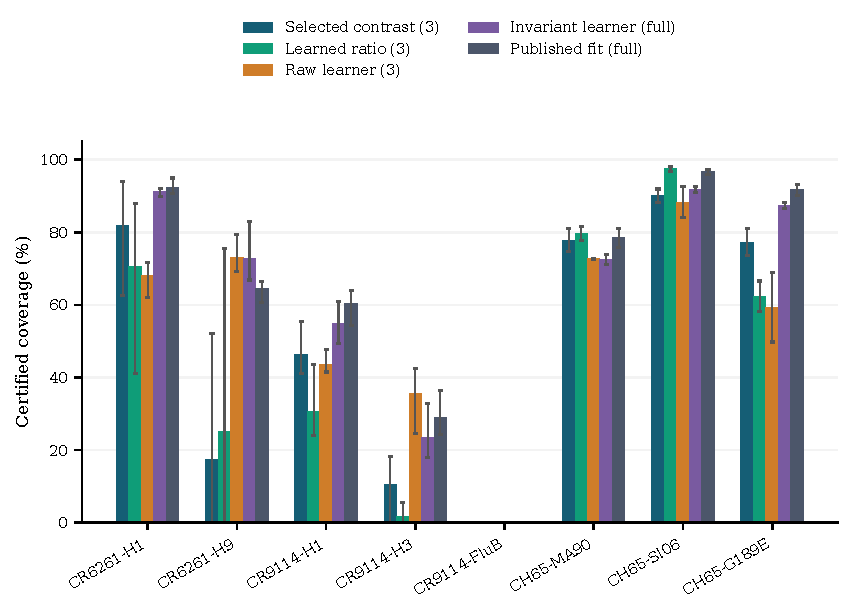
\includegraphics[width=\linewidth]{figures/coverage.pdf}
\caption{Certified coverage by task and readout. Bars show means over the source configurations and five split seeds; thin ranges show the minimum and maximum configuration-level seed mean. Coverage is conditional on the evaluable cohort, not the original library. The full panel contains 12 conditions in the CR tasks and 10 in CH65. All methods use the same gate-validation procedure.}
\label{fig:coverage}
\end{figure}

\subsection{Acceptance does not imply high hit recovery}
\ResultsRecall

\begin{figure}[t]
\centering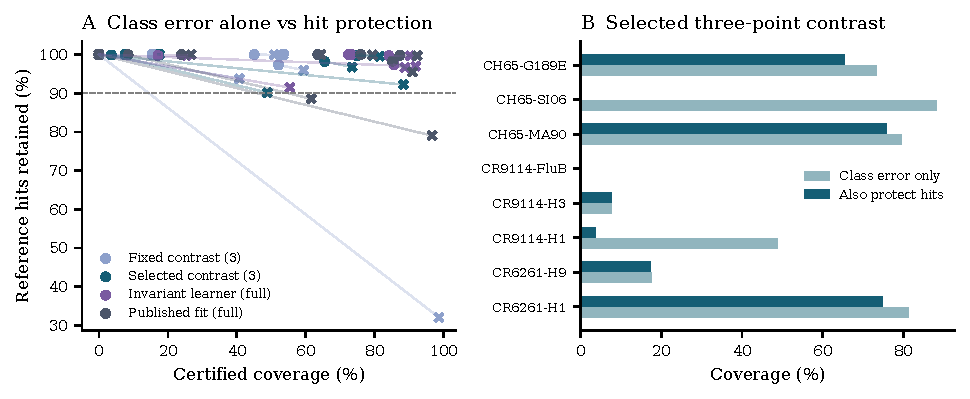
\includegraphics[width=\linewidth]{figures/hit_protection.pdf}
\caption{Hit protection changes the scientific objective. Crosses denote class-error control alone; circles additionally bound the fraction of hits discarded as negatives. Lines join matched method/task means over three split seeds. Right: the selected three-point contrast can lose most of its certified coverage when it must also protect rare hits. Complete deferral retains all hits for further measurement, but identifies none.}
\label{fig:protect}
\end{figure}


This distinction matters commercially. A workflow that safely declines to certify most positives may protect the precision of the few accepted hits while contributing little to discovery. We therefore retain hit recall alongside coverage and accepted error, rather than presenting only an accuracy figure. The eight tasks also share antibody families and experimental procedures; they are not eight independent demonstrations of broad biological generalization.

\subsection{Affine invariance is measurable, but not a universal robustness claim}
\begin{table}[t]
\centering\footnotesize
\caption{Constructed affine stress: forced decision changes (\%) and accepted error (\%) for raw-input learners. Invariant readers have zero decision changes. Dashes denote no accepted decisions.}
\setlength{\tabcolsep}{4pt}
\begin{tabular}{lrrrrr}
\toprule
Task & Raw 3 flip & Raw full flip & Raw 1 flip & Full error & Stressed \\
\midrule
CR6261-H1 & 22.2 & 23.8 & 19.0 & 0.9 & 20.4 \\
CR6261-H9 & 21.7 & 21.0 & 19.7 & 1.0 & 13.0 \\
CR9114-H1 & 30.3 & 30.7 & 28.1 & 3.2 & 12.8 \\
CR9114-H3 & 32.0 & 35.0 & 29.7 & 2.9 & 31.0 \\
CR9114-FluB & 38.4 & 38.5 & 37.0 & -- & -- \\
CH65-MA90 & 19.3 & 23.9 & 39.3 & 0.4 & 13.5 \\
CH65-SI06 & 29.0 & 25.9 & 16.0 & 0.1 & 1.1 \\
CH65-G189E & 23.6 & 27.4 & 20.9 & 2.6 & 23.1 \\
\bottomrule
\end{tabular}
\end{table}

\ResultsStress

An invariant full-panel learner is a necessary comparator: nuisance robustness is not unique to a sparse panel or to the zero-contrast rule. The three-point ratio can preserve the same type of invariance with fewer input conditions, while additional concentrations may improve error ranking and coverage. Neither result addresses concentration-dependent drift, changes in antigen valency, heterogeneous binding populations, or a change in the underlying affinity itself.

\begin{figure}[t]
\centering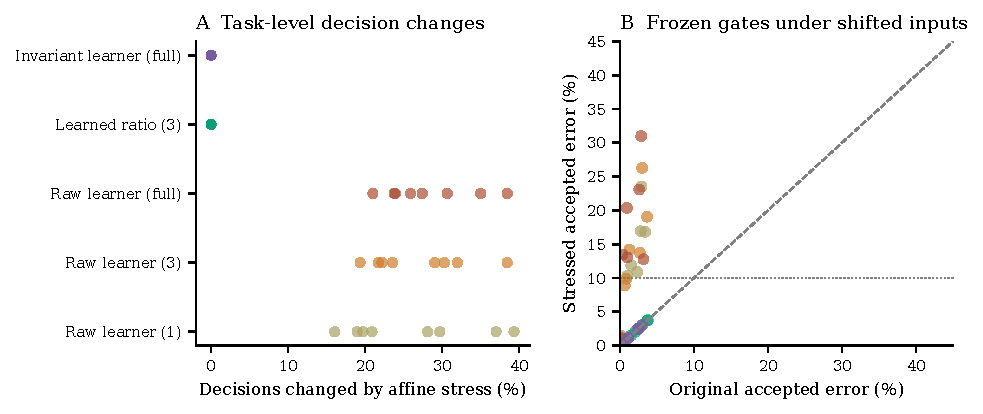
\includegraphics[width=\linewidth]{figures/stress.pdf}
\caption{Constructed affine robustness test. Left: changes in forced decisions after test-only gains and offsets, with models frozen. Right: accepted error before and after the same perturbation. Ratio and invariant-panel decisions are unchanged up to numerical precision. The perturbation is synthetic; the underlying unperturbed inputs and reference outcomes are measured data.}
\label{fig:stress}
\end{figure}

\subsection{Reference budgets and threshold choices change feasibility}
\ResultsSensitivity

\begin{figure}[t]
\centering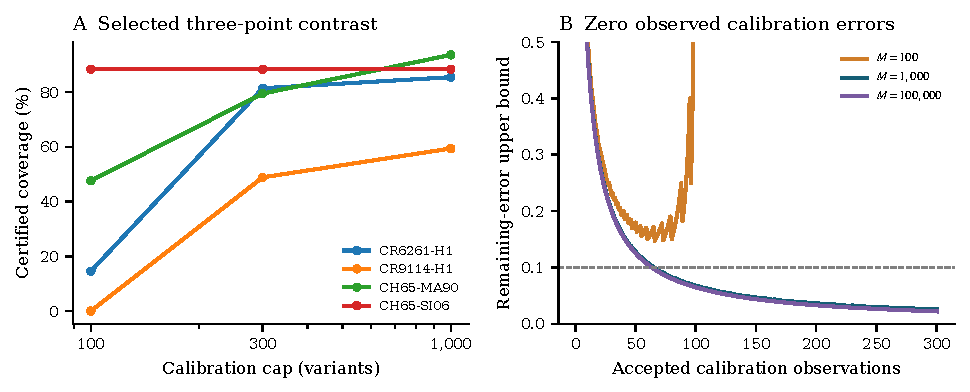
\includegraphics[width=\linewidth]{figures/validation.pdf}
\caption{Validation cost. Left: certified coverage as the calibration cap changes, using three split seeds and unchanged development rules. Right: the exact remaining-error upper bound for an error-free accepted calibration sample, at $\delta/40$, for illustrative accepted population sizes. This theoretical calculation explains why a small reference cohort can produce complete deferral even when observed predictions are often correct.}
\label{fig:validation}
\end{figure}

\section{Implications for discovery systems and commercial use}
\paragraph{A measurement contract for a scientific tool.}
A tool should return the declared threshold, concentrations, source observations, readout version, calibration membership, error bound, and defer status. An orchestration model may propose a panel or request a follow-up, but a textual assertion of confidence does not replace this evidence. A useful integration would expose a deterministic decision tool whose output is inspectable by both a scientist and an agent. The present work implements the numerical core, not a tested language-model orchestration system.

\paragraph{Economic unit and amortization.}
Three input conditions are not a demonstrated 75\% reduction in laboratory cost. In pooled Tite-Seq, a condition measures the whole pool; sorting, sequencing, controls, pilot construction, and reference measurements have costs that differ from per-variant prediction cost. Selecting a panel from complete development curves requires a historical campaign or a separately assayed pilot pool. Running all development conditions on the same full pool and then discarding measurements yields no experimental saving. If a reusable pilot requires $C$ conditions and $J$ later campaigns use three each, a simplified condition count is $C+3J$, compared with $CJ$ full-panel conditions; reference and operational costs must still be added. This is an accounting identity, not an observed saving.

\paragraph{Position in an existing market.}
Commercial providers already distinguish quick binding screens from full affinity characterization \citep{adaptyv}, while integrated discovery platforms combine design with laboratory feedback \citep{absci}. A plausible product opportunity is validation and assay-decision infrastructure between these components, rather than claiming to have invented automated protein discovery. The evidence here supports a prototype and a prospective evaluation plan. It supplies no revenue estimate, customer validation, service-level guarantee, or patent assessment.

\section{Limitations and next experiments}
The evidence is retrospective and limited to three related antibody families in two published studies. Reference labels are noisy assay-derived quantities; two-day consensus is not physical ground truth, and CH65 uses only one reference day. Filtering on reference fit quality creates an evaluable cohort that can be much smaller than the original library. In particular, the influenza-B result cannot be extrapolated to its unmeasured or poorly fitted variants. Prospective deployment would need to identify unresolved cases and pay for additional evidence.

The response model assumes one-site equilibrium binding with concentration-independent amplitude and background. Yeast-displayed antibodies and multivalent antigens need not follow that model exactly; quantitative binding work requires explicit checks of assay assumptions \citep{jarmoskaite2020}. Ratios can amplify small-denominator noise; the declared clipping rule can also lose information. Isotonic learning can improve a library-specific boundary without restoring a physical interpretation. The affine stress test covers one mathematical nuisance family, with appropriately transformed noise scales, and is not a wet-lab test of expression drift.

Calibration uses random sampling from a fixed library. Applying the same certificate after adaptive sequence generation, selective reference acquisition, or a new assay day requires a different sampling argument or a fresh audit. Thresholds and development choices were exploratory. A stronger external test would freeze them before receiving new data and include non-antibody targets, additional instruments, and prospective batch costs.

A feasible follow-up is to freeze a sparse panel and its readout on an existing antibody reference set, measure that panel and a full curve on the same new library, and compare accepted error and recovered hits on independent days. Expression and background perturbations should be separately controlled rather than inferred from amplitude correlations. The primary endpoint should be class-specific accepted error at a declared coverage and total experimental budget. Quine's model, tool, and experimental-feedback setting is a natural environment for that follow-up \citep{quine}; access or experimental support has not been obtained for this study.

\section{Conclusion}
A sparse titration can support a precise affinity decision without identifying every response parameter, but algebraic sufficiency, empirical prediction, and statistical validation are distinct requirements. Measured replicate data show substantial differences across targets and source days, including settings where all methods must defer. Affine-invariant readouts preserve decisions under a specified nuisance transformation; they do not remove measurement noise or the cost of reference validation. The resulting workflow makes those boundaries executable and provides a reproducible basis for prospective assay-design research.

\paragraph{Data and code availability.}
All experimental observations originate from the cited public studies. The artifact contains pinned download manifests, analysis and figure code, full primary run summaries, held-out predictions, sensitivity results, and verification tests. No simulated observation is mixed into the measured-data results. Computational perturbations are labeled separately.

\bibliographystyle{unsrtnat}
\bibliography{references}

\appendix
\section{Reproducibility and audit details}\label{app:repro}
\noindent\textbf{2021 study.} Repository: \texttt{klawrence26/bnab-landscapes}.\\
Commit: \texttt{514d62f387070f43b8a172f02e60c70137f8a8b8}.

\noindent\textbf{2023 study.} Repository: \texttt{amphilli/CH65-comblib}.\\
Commit: \texttt{cea336dfd05fa31d675f79038428bf7f0d177e78}.

The manifests record exact source paths, byte counts, and SHA-256 hashes. Genotypes are read as strings to retain leading zeroes and are joined by identifier rather than row position.

For CR6261 and CR9114, each headerless mean-response table contains a genotype, 12 log-responses, and 12 spreads. The separate fit table contains the genotype, $-\log_{10}\KD$, amplitude, background, fit $r^2$, fit uncertainty, and curve observations. For CH65, exported \texttt{mean\_log10PE0} is the blank and columns 1--9 are positive concentrations; sample metadata fixes their values. The loader reorders them to positive concentrations followed by the blank. This handling is checked against published fit parameters and stored $r^2$, rather than inferred from a visually plausible curve.

\VerificationText

Primary results comprise eight methods, five random splits, and 21 source/reference configurations. The sensitivity analyses are reported separately and use three seeds. The experimental unit for source-day variation is the source/reference configuration; repeated genotype partitions are computational resamples. All tabulated means weight configurations and seeds equally within a task. They do not pool millions of correlated predictions into an artificial biological sample size.

\section{Algorithm and operational output}
For a declared task, first define the reference label and the evaluable population. Reserve development variants independently of the remaining calibration/test split. Fit the panel and readout using only development outcomes. Freeze their implementation and the two margin grids. Observe source features for the remaining population; select a simple random calibration sample and acquire its reference outcomes. For each class and margin, count accepted population size, accepted calibration size, and calibration errors. Invert the hypergeometric lower tail by integer binary search, and select the largest qualifying accepted remainder. Return its certificate and defer elsewhere.

The finite-population calculation uses logarithmic cumulative probabilities to avoid underflow. When there are no accepted calibration examples, the bound is one. When the accepted test set is empty, the gate contributes no useful coverage. Selection is simultaneous over all 40 declared gates, including duplicates; this conservative correction is retained in every method. A zero-confidence score is not automatically treated as trustworthy: it must pass the same calibration gate.

\section{Additional numerical results}
\begin{table}[t]
\centering\footnotesize
\caption{Balanced error if every prediction were forced (\%).}
\setlength{\tabcolsep}{4pt}
\begin{tabular}{lrrrrrrrr}
\toprule
Task & \shortstack{Fixed\\3} & \shortstack{Selected\\3} & \shortstack{Ratio\\3} & \shortstack{Raw\\3} & \shortstack{Raw\\1} & \shortstack{Raw\\full} & \shortstack{Invariant\\full} & \shortstack{Fit\\full} \\
\midrule
CR6261-H1 & 9.6 & 5.9 & 5.9 & 5.1 & 5.5 & 3.8 & 3.5 & 5.4 \\
CR6261-H9 & 27.3 & 26.7 & 35.3 & 5.8 & 5.4 & 4.7 & 5.9 & 27.1 \\
CR9114-H1 & 29.3 & 24.7 & 34.9 & 25.6 & 28.0 & 22.2 & 20.3 & 25.8 \\
CR9114-H3 & 33.9 & 18.3 & 19.0 & 13.7 & 14.8 & 11.1 & 15.3 & 14.4 \\
CR9114-FluB & 36.7 & 29.6 & 32.2 & 20.2 & 23.0 & 15.7 & 25.0 & 19.3 \\
CH65-MA90 & 15.5 & 5.8 & 7.0 & 5.6 & 26.5 & 4.4 & 4.1 & 5.4 \\
CH65-SI06 & 39.6 & 8.4 & 27.0 & 6.2 & 6.6 & 4.6 & 4.5 & 13.2 \\
CH65-G189E & 24.5 & 8.4 & 8.6 & 10.2 & 10.5 & 7.0 & 5.9 & 5.1 \\
\bottomrule
\end{tabular}
\end{table}

\begin{table}[t]
\centering\footnotesize
\caption{Reference hits retained for positive identification or further testing (\%). Only accepted negatives discard a hit.}
\setlength{\tabcolsep}{4pt}
\begin{tabular}{lrrrrrrrr}
\toprule
Task & \shortstack{Fixed\\3} & \shortstack{Selected\\3} & \shortstack{Ratio\\3} & \shortstack{Raw\\3} & \shortstack{Raw\\1} & \shortstack{Raw\\full} & \shortstack{Invariant\\full} & \shortstack{Fit\\full} \\
\midrule
CR6261-H1 & 99.8 & 99.4 & 99.5 & 99.8 & 99.9 & 99.6 & 99.4 & 99.6 \\
CR6261-H9 & 100.0 & 100.0 & 100.0 & 99.9 & 99.9 & 99.9 & 100.0 & 100.0 \\
CR9114-H1 & 92.7 & 91.3 & 96.3 & 93.8 & 94.8 & 91.3 & 91.4 & 89.4 \\
CR9114-H3 & 100.0 & 100.0 & 100.0 & 100.0 & 99.8 & 99.3 & 99.8 & 100.0 \\
CR9114-FluB & 100.0 & 100.0 & 100.0 & 100.0 & 100.0 & 100.0 & 100.0 & 100.0 \\
CH65-MA90 & 100.0 & 99.8 & 99.8 & 99.9 & 100.0 & 100.0 & 100.0 & 99.9 \\
CH65-SI06 & 29.8 & 91.1 & 51.7 & 96.4 & 95.8 & 95.7 & 96.6 & 78.3 \\
CH65-G189E & 95.9 & 95.5 & 96.4 & 95.9 & 96.2 & 96.6 & 96.7 & 95.6 \\
\bottomrule
\end{tabular}
\end{table}

\begin{table}[t]
\centering\footnotesize
\caption{Selected three-point contrast with and without the hit-protection certificate (\%). Matched comparison uses three seeds. With hit protection, the confidence correction also includes complementary-stratum count bounds.}
\setlength{\tabcolsep}{4pt}
\begin{tabular}{lrrrr}
\toprule
Task & Base coverage & Hits retained & Protected coverage & Hits retained \\
\midrule
CR6261-H1 & 81.4 & 99.6 & 74.9 & 99.7 \\
CR6261-H9 & 17.5 & 100.0 & 17.3 & 100.0 \\
CR9114-H1 & 48.9 & 90.1 & 3.6 & 99.9 \\
CR9114-H3 & 7.7 & 100.0 & 7.7 & 100.0 \\
CR9114-FluB & 0.0 & 100.0 & 0.0 & 100.0 \\
CH65-MA90 & 79.5 & 99.7 & 75.8 & 100.0 \\
CH65-SI06 & 88.4 & 92.2 & 0.0 & 100.0 \\
CH65-G189E & 73.4 & 96.8 & 65.5 & 98.2 \\
\bottomrule
\end{tabular}
\end{table}

\begin{table}[t]
\centering\footnotesize
\caption{Selected-contrast coverage (\%) under declared sensitivity settings; three seeds each. Cal = calibration cap; cut $\pm0.5$ = shift in log-affinity cutoff; risk = class-specific target $\alpha$.}
\setlength{\tabcolsep}{4pt}
\begin{tabular}{lrrrrrr}
\toprule
Task & Cal 100 & Cal 1,000 & Cut $-0.5$ & Cut $+0.5$ & Risk 5\% & Risk 20\% \\
\midrule
CR6261-H1 & 14.5 & 85.5 & 74.6 & 78.2 & 32.3 & 97.1 \\
CR6261-H9 & 0.0 & 17.6 & 57.7 & 67.4 & 11.4 & 38.0 \\
CR9114-H1 & 0.0 & 59.4 & 69.6 & 99.7 & 0.0 & 63.2 \\
CR9114-H3 & 0.0 & 26.3 & 36.6 & 47.8 & 0.0 & 45.7 \\
CR9114-FluB & 0.0 & 0.0 & 0.0 & 0.0 & 0.0 & 0.0 \\
CH65-MA90 & 47.6 & 93.6 & 92.2 & 85.1 & 71.5 & 91.8 \\
CH65-SI06 & 88.4 & 88.4 & 75.1 & 99.3 & 88.4 & 88.4 \\
CH65-G189E & 0.0 & 91.7 & 55.1 & 70.0 & 7.0 & 96.1 \\
\bottomrule
\end{tabular}
\end{table}


\end{document}
